\chapter{Data wrangling and organizing}
Now that we have a defined business problem, in this section we need to dig deeper into the dataset we received from our client. In addition to exploring the given dataset numerically and graphically, we need to ensure whether the dataset makes sense and matches to what we were told by our client, in this case to what is written on UCI website. The main
 focus of Data wrangling is organizing and cleaning our dataset making it ready for building the best performing Machine Learning model. In what follows below are essential guiding questions that need to be addressed during data wrangling and exploration:

\begin{itemize}
    \item How many samples (rows)?
\item How many features (columns)
\item Types of features? - Which are Categorical? Which are numerical?
\item What Does the features data look like?
\item Range of values for numeric features
\item Frequency of classes for categorical features
\item Are there any missing values?

\end{itemize}
\section{Size and type of dataset}
After loading our dataset into a dataframe {\color{blue} df}, we obtained the number of rows and columns with the following pandas commands. 
\begin{verbatim*}
df = pd.read_csv('bank-full.csv')
df.shape
output:(45211, 17)
\end{verbatim*}
As can be seen from the output above our loaded dataset consists of 45211 rows and 17 columns which was also confirmed by loading the dataset with an excel spreadsheet. 

As can be seen from the output of the pandas code below, our data set consists of 17 features with 7 integer type features and 10 object type (categorical features). In what follows below is a list of the 7 integer type features and 10 categorical features. 

\begin{verbatim}
    Integers: ['age','balance', 'day', 'duration', 'campaign', 'pdays', 'previous']
    Categorical:['job', 'marital', 'education', 'default', 'housing', 'loan', 
    'contact', 'month', 'poutcome', 'Target']
\end{verbatim}

\section{Visualizing the categorical features}

In this section we want to understand how many unique values each of the categorical features possess and how many customers with each categorical feature values were contacted by the bank. For ease of our analysis the categorical features were grouped into demographic, financial, and campaign.

\subsection{Visualizing demographic distribution of customers}
Demographic segmentation is a commonly used technique in marketing where target categories based on one or more of socio-economic variables like job, age, gender, marital status, income, education, etc. In our case the categorical demographic content of the customers contacted by the bank includes \hl{job, marital, education}.

The customer distribution contacted by the bank during this telemarketing campaign for each customer demographic category is shown in figure \ref{fig:cat_demo_count}.

\begin{figure}[tbh]
\centering
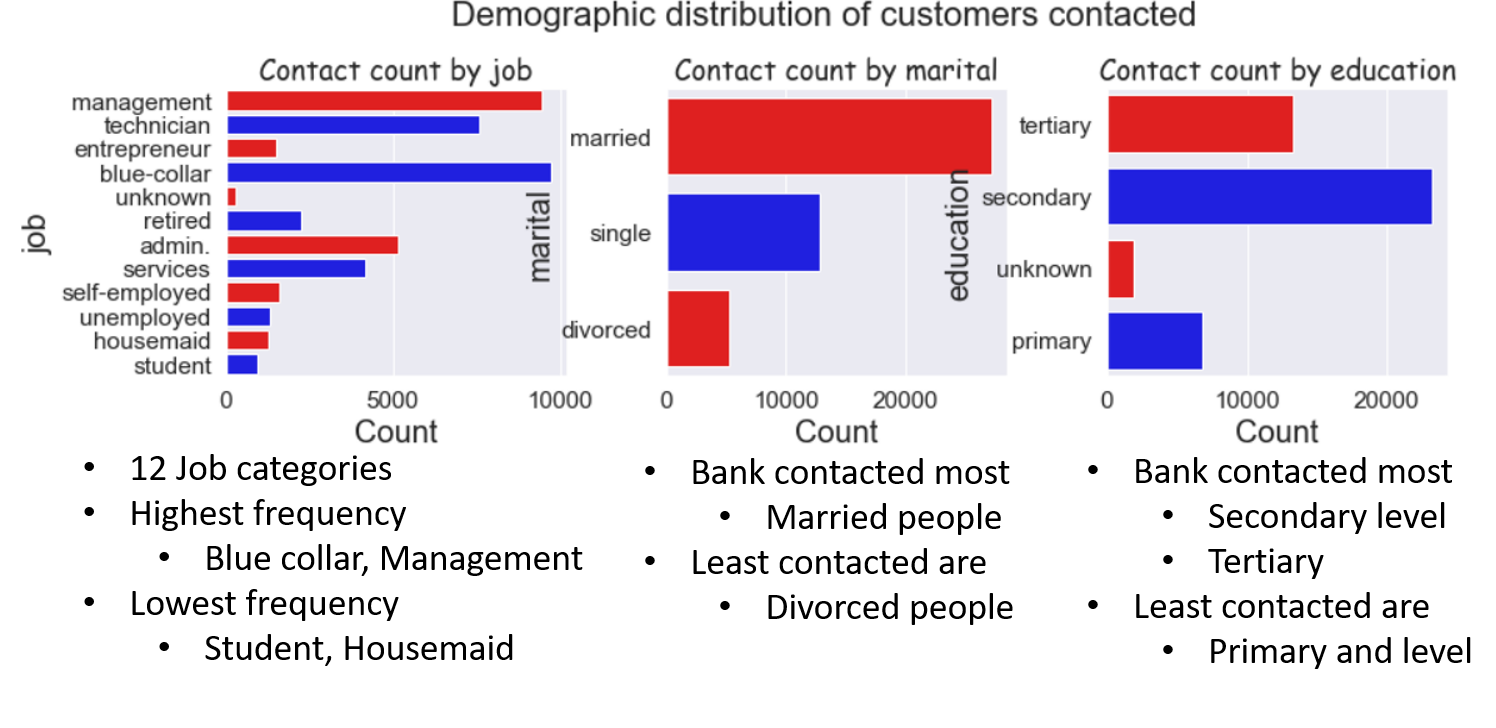
\includegraphics[width = 1.0\hsize]{./resources/img/fig_cat_demo_count.png}
\caption{Frequency of customers contacted by the bank during the telemarketing for each job category, marital status, and educational level.} 
\label{fig:cat_demo_count}
\end{figure}

\subsubsection*{Customer jobs}
Customers with {\color{blue} \textbf{blue-collar}} jobs were contacted the most during the marketing campaign. Customer's whose jobs is unknown (either not recorded or customer did not want to specify) are targeted the least during the marketing campaign. Following customers with blue-collar managers, technicians, and administrators, respectively in decreasing order were contacted during the marketing campaign. As one might expect students were targeted the least during the marketing campaign.

\subsubsection*{Marital status}
Marital status is another important trait used in demographic segmentation. It provides useful information to target audience during marketing communication through promotional messages. Usually people in the same marital status group have common tastes and can can be easily targeted based on marital status. For example, generally people who are married need more financial strategy and are likely expected to respond to the term deposit marketing campaign. The largest number of people contacted during the marketing campaign are married. The list contacted people are divorced individuals.

\subsubsection*{Educational level}

The level of education of an individual is also an important trait when segmenting population for marketing campaigns. For example educational level determines the choice of communication channel in passing across your message. During the marketing campaign customer who completed high school are contacted the most. There are also a few number of contacts made where customer's education level is UNKNOWN.

\subsection{Visualizing financial data segmented distribution of customers}
In addition to demographic segmentation, customers could be grouped together based on their account related to their finances. That is whether a customer has credit or not (`default`), has housing loan or not (`housing`), and has personal loan or not (`loan`).  In figure \ref{fig:cat_financial_count} we plot the distribution of customers segmented by their financial status.   


\begin{figure}[tbh]
\centering
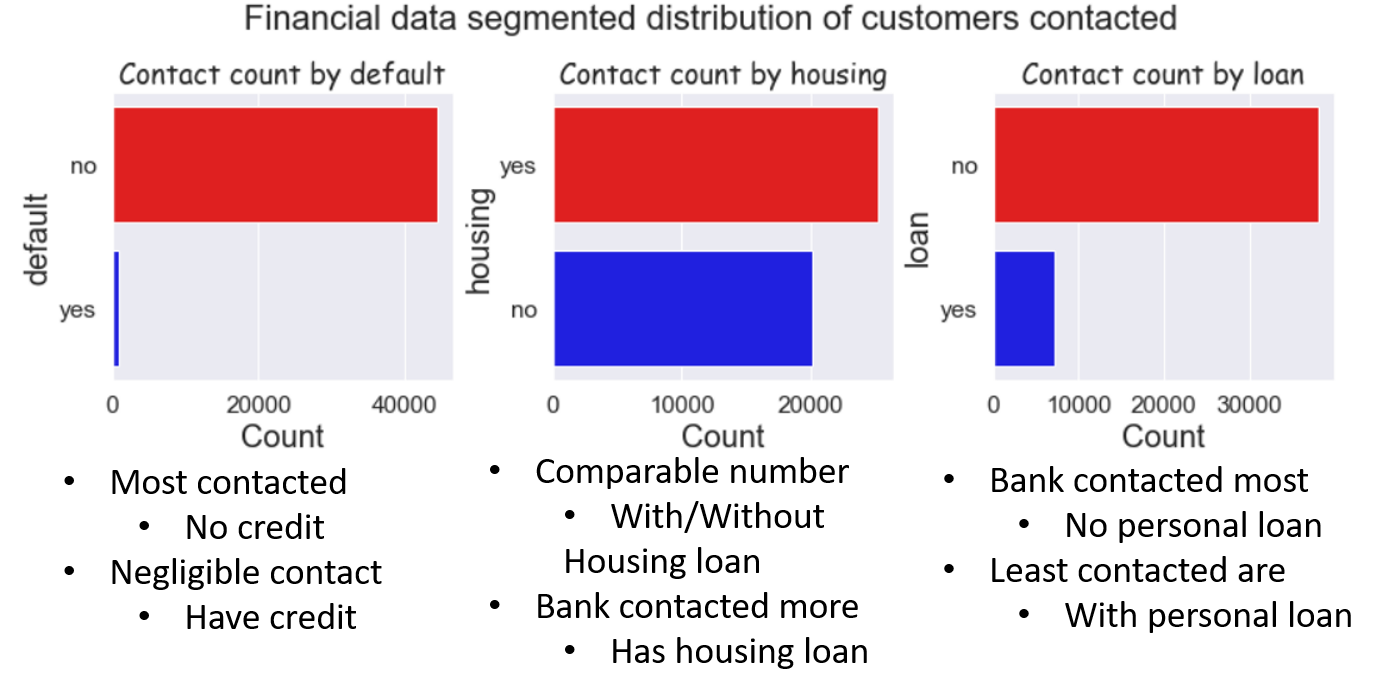
\includegraphics[width = 1.0\hsize]{./resources/img/fig_cat_financial_count.png}
\caption{Frequency of customers contacted by the bank during the telemarketing for customers with/without credit, housing loan, and personal loan.} 
\label{fig:cat_financial_count}
\end{figure}

\subsubsection*{Has credit (default)}
Majority of customers contacted by the bank do not have credit or did not default (98.2\%). Only a few fraction (1.8\%) of all the customers contacted had credit. Hence, credit might not be an important feature in determining whether a customer will subscribe to a term deposit or not. 

\subsubsection*{Housing loan}
During this telemarketing campaign, the bank called an almost balanced number of customers depending whether they have housing loan or not. About 55\% of the customers contacted by the bank during this telemarketing possess housing loan. The remaining about 45\% of the customers contacted did not have housing loan.

\subsubsection*{Personal loan}
The majority of customers (84\%) called during this telemarketing did not have any personal loans. However, a non-negligible number of customers (16\%) had personal loans.

\subsection{Distribution of customers versus past and current campaign details}
In addition to demographic and financial segmentation, customers could be grouped together based on the details of the past and present campaign parameters.  That is how was the customer contacted (for example iPhone or phone), the particular month the customer was contacted and the what was the outcome of the previous telemarketing campaign? 

In figure \ref{fig:cat_campaign_count} we plot customers segmented by details of the past and present campaign.  


\begin{figure}[tbh]
\centering
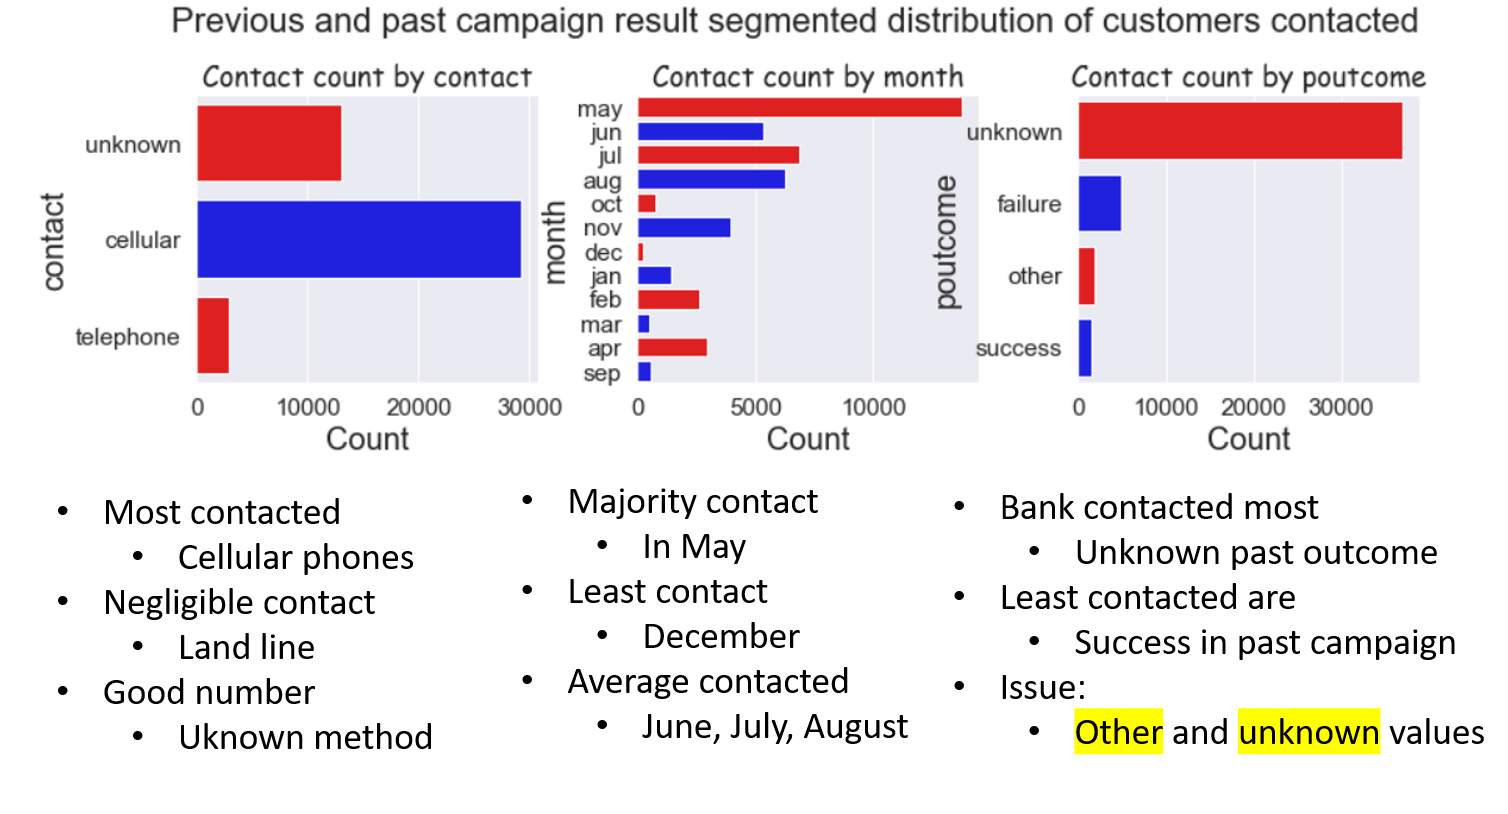
\includegraphics[width = 1.0\hsize]{./resources/img/fig_cat_campaign_count.png}
\caption{Frequency of customers contacted by the bank during the telemarketing for each method of contact, contact month, and outcome of previous telemarketing.} 
\label{fig:cat_campaign_count}
\end{figure}

\subsubsection*{Method of contact}
During this telemarketing, the majority of the customers (65\%) were contacted using cellular phones. While contacts made through land lines amounted only to 6.5\%, a significant fraction of customers (29\%) were contacted through mode of communication that was not registered and marked as unknown. Different segments of the populations prefer different methods of contact. The communication channel used during the marketing campaign is essential. The largest number of customers were contacted through cellular phone. The least popular method of contact was through telephone. During the marketing campaign, 65\% of the population contacted by the bank was through cellular phones. Only 6.4\% contacted through a telephone line while about 29\% contacted through an unknown (unspecified) mode of communication.

\subsubsection*{Month customer contacted}

The season when the bank should contact target population segment is also an important trait for the success of the marketing campaign. The largest number of contacts were made during spring and summer seasons with combined contact rate of 79 \%. This is understandable since spring and summer are the beginning and end dates of the tax season; where customers may be motivated for financial plans due to expected tax returns. Barely any telemarketing was conducted during the winter which is understandable as it is the holiday and end of year season. However, whether the choice of these high contact seasons maximizes efficiency requires farther analysis and will be discussed during the exploratory data analysis part of this project.  

\subsubsection*{Previous marketing outcome}
During this telemarketing, 3.3\% of all the customers contacted have subscribed in a previous campaign while 10.8\% did not subscribe in the past. The bank decided to contact more customers who did not subscribe in the past.  

- \hl{\textbf{`Issue:`}}

There are two ambiguous values in this feature, namely `unknown` and `other`. We need to change the `unknown` to `other` for ease of analysis and doing so does not change anything since `unknown` is practically `other`.

\subsection{Class imbalance}
To determine whether we are dealing with a balanced dataset or we have to deal with the difficulties in model evaluation for an imbalanced dataset, we need to look at the fraction of the two target classes, namely: 1) term-deposit subscribed 2.) term-deposit NOT subscribed. 

In figure \ref{fig:target_imbalance} we plot the distribution of the two classes for our dataset. 

\begin{figure}[tbh]
\centering
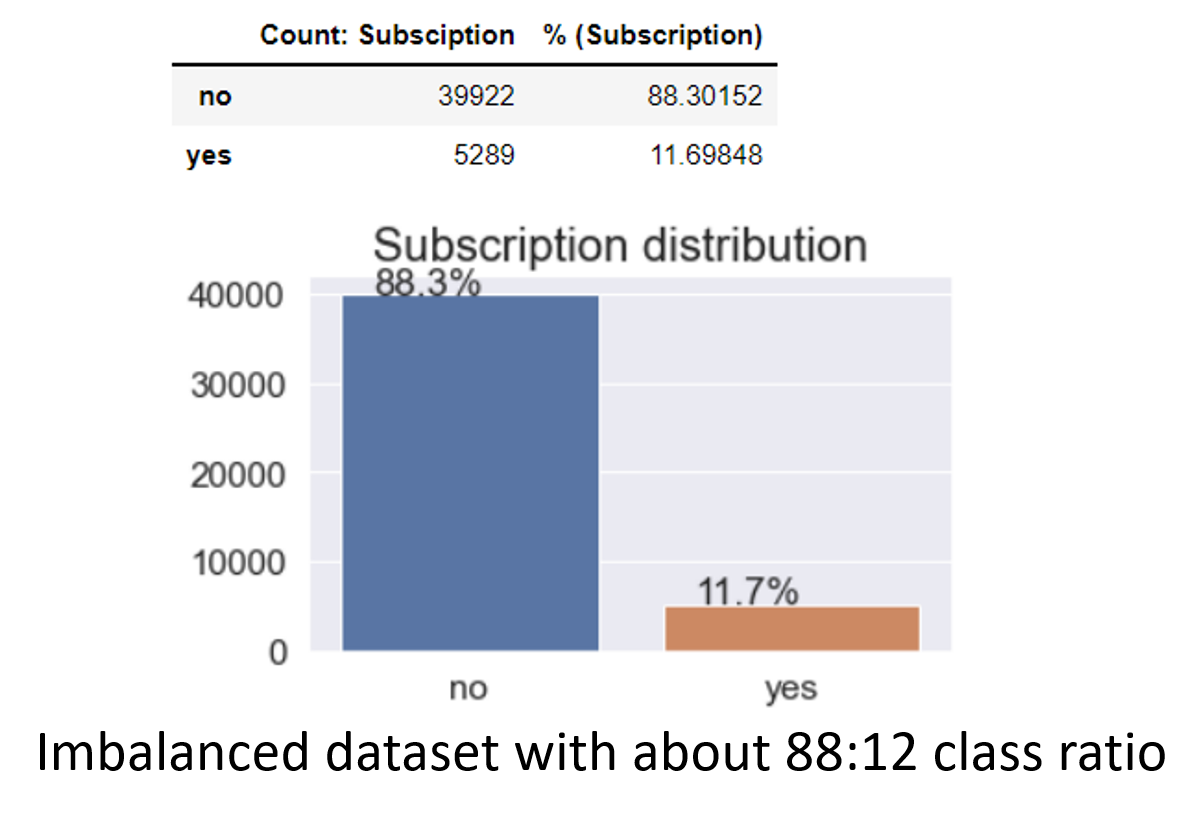
\includegraphics[width = 0.7\hsize]{./resources/img/fig_target_imbalance.png}
\caption{Frequency of the two target classes revealing an imbalanced dataset.} 
\label{fig:target_imbalance}
\end{figure}
\\

\section{Range of numerical features}
Let us know turn to investigating the range and type of the numerical features of our dataset. 

\subsection{Age range and account balance}

The number of customers contacted during this telemarketing by the range of customer ages as well as their account balance is shown in figure \ref{fig:age_balance_count}.

\begin{figure}[tbh]
\centering
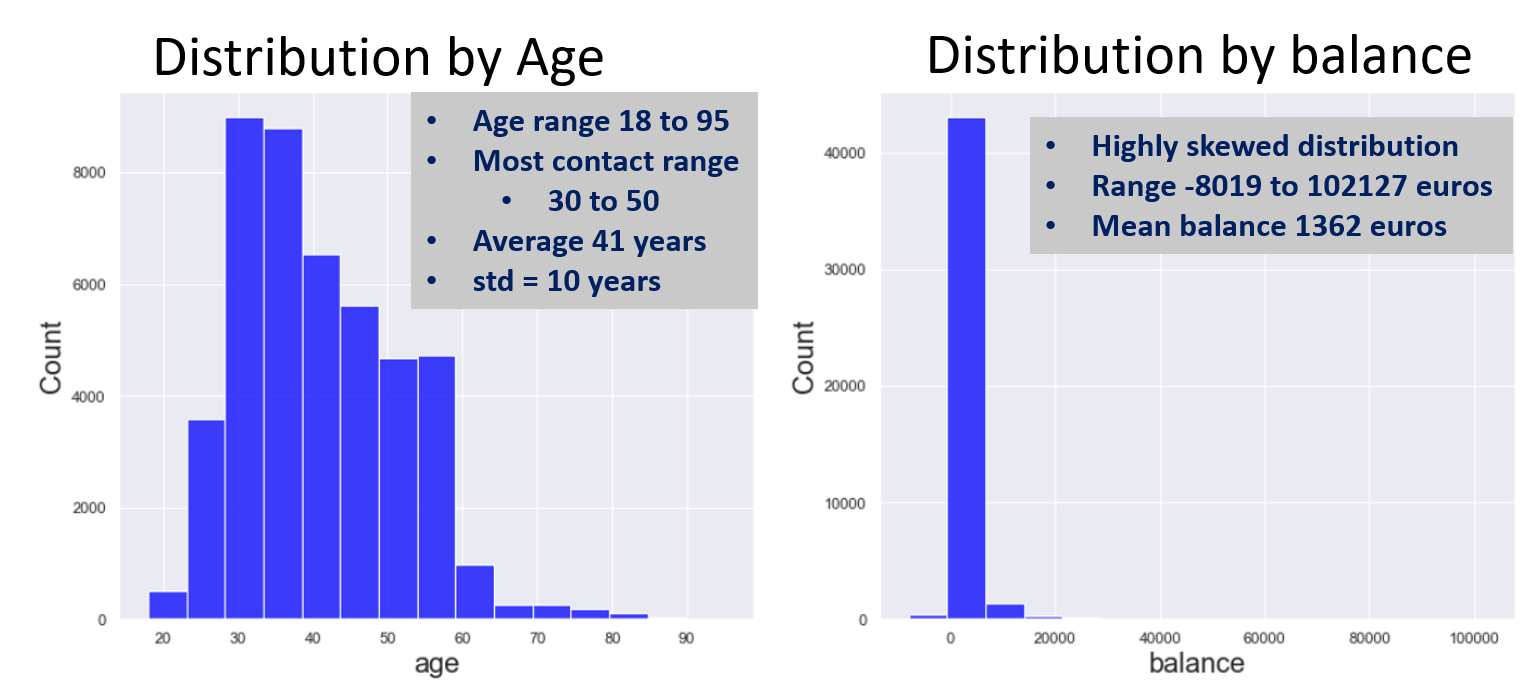
\includegraphics[width = 0.7\hsize]{./resources/img/fig_age_balance_count.png}
\caption{Frequency customers contacted during this telemarketing per age and account balance.} 
\label{fig:age_balance_count}
\end{figure}

\subsubsection*{Distribution of age}
The age of customers contacted by the bank during the telemarketing extends from a minimum age of 18 years to a maximum age of 95 years old. The majority of customer contacted by the bank were in their 30s and 40s (33 to 48 years land within $25^{th}$ and $75^{th}$ percentiles). With an average age of 41 years old and a standard deviation of 10 years, the distribution of age is close to normal distribution.

\subsubsection{Distribution of balance}
The customers contacted include those with positive and negative account balances. The distribution of account balances is highly skewed. The account balance of the customers called by the bank extends from -8019.0 to 102127.0 euros, resulting to a range of 110146 euros. With a mean of 1362 euros and standard deviation of 3044 euros, the balance distribution is highly skewed and far from normal. There are significant number of ateliers as can be seen by looking how far the minimum and maximum values from the mean. 

To see the inter-dependence of age on balance, a scatter plot of age versus account balance is shown in figure \ref{fig:age_balance_scatter}. The figure shows no clear dependence of account balance on the customer's age. However, in general customers over the age of 60 and less than 20 years old seem to possess smaller account balances. This may be due to the fact the younger customers are in the process of establishing themsleves while the older customers have already retired and may not have any reliable source of income.


\begin{figure}[tbh]
\centering
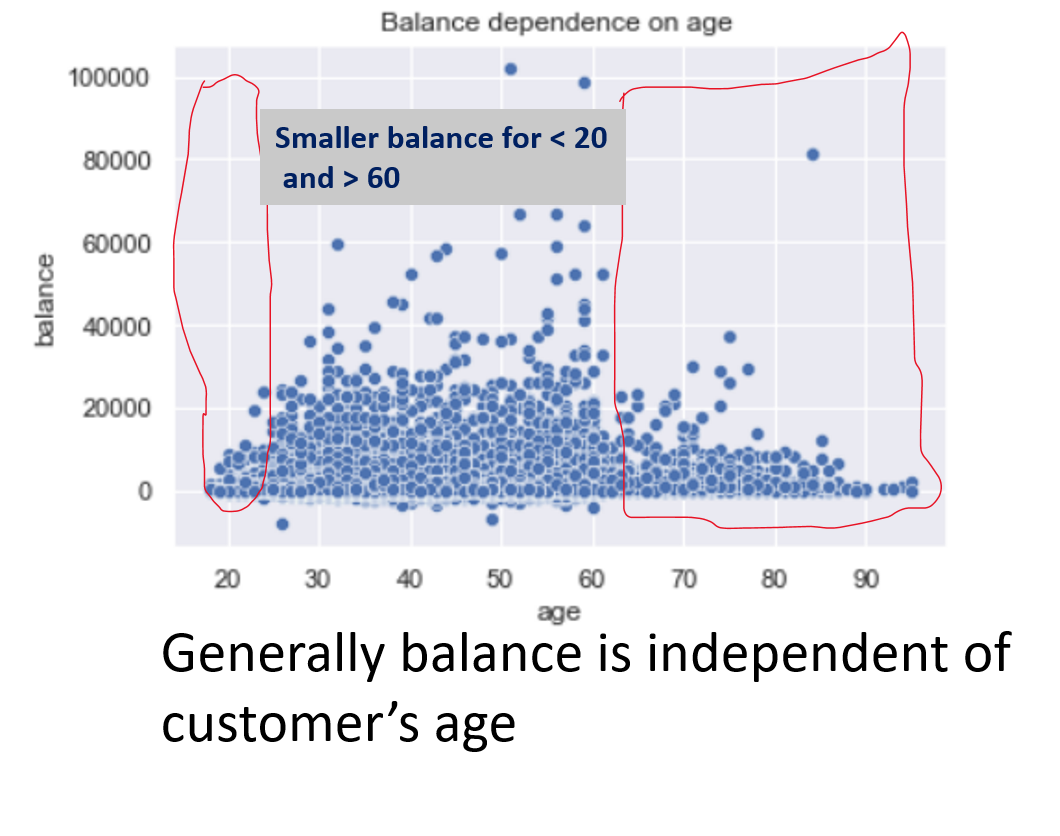
\includegraphics[width = 0.7\hsize]{./resources/img/fig_age_balance_scatter.png}
\caption{Customer age versus account balance.} 
\label{fig:age_balance_scatter}
\end{figure}

\subsection{Duration of contact and number of contacts}
The distribution of the duration of contact in minutes and the number of contacts is shown in figure \ref{fig:duration_campaign_count}

\begin{figure}[tbh]
\centering
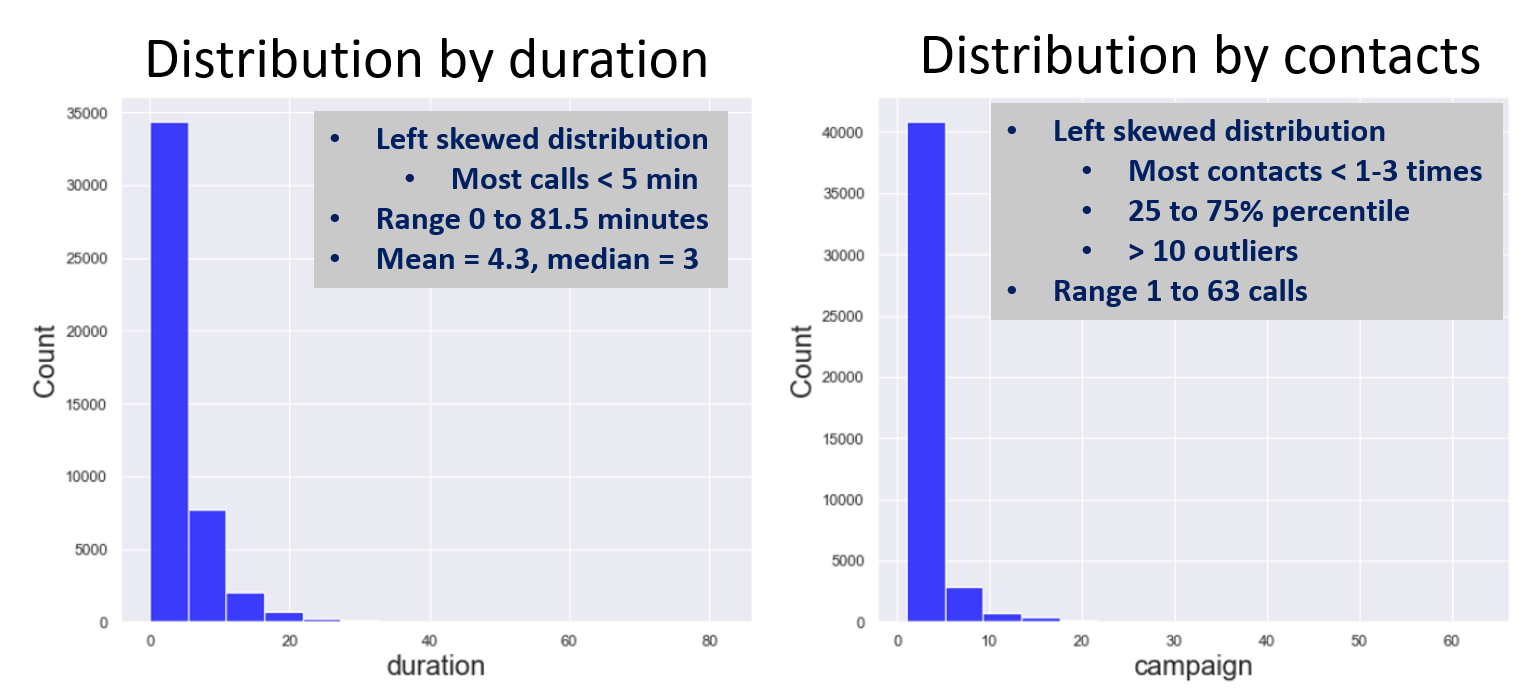
\includegraphics[width = 0.8\hsize]{./resources/img/fig_duration_campaign_count.png}
\caption{Customer age versus account balance.} 
\label{fig:duration_campaign_count}
\end{figure}

\subsubsection*{Distribution of duration}
The duration of a phone call made during the telemarketing extends from a minimum of 0 minutes to a maximum of 81.9 minutes. With mean duration of 4.3 minutes and median duration of 3 minutes, the distribution of the duration of all the calls during the telemarketing is left skewed; meaning most of the calls are of short duration, typically less than 5 minutes.

\subsubsection*{Distribution of campaign}
The number of contacts performed during this campaign and for this client is plotted in the histogram plot shown above. The number of contacts made a client ranged from a minimum of 1 call to an extreme maximum of 63 calls. However, the majority of the calls required 1 to 3 contacts only (25 percentile to 75 percentile); indicating contacts more than 10 are outliers in the distribution.

To see whether the duration of contact is the result of many contacts, in figure \ref{fig:duration_campaign_scatter} we show a scatter plot of duration versus number of contacts. Generally, the call duration decreases as the number of contacts during the campaign increases. The largest number of contacts made resulted to lowest call duration. 

\begin{figure}[tbh]
\centering
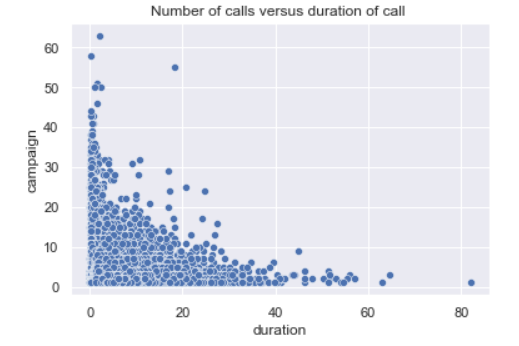
\includegraphics[width = 0.8\hsize]{./resources/img/fig_duration_campaign_scatter.png}
\caption{Customer age versus account balance.} 
\label{fig:duration_campaign_scatter}
\end{figure}

\subsection{Correlation matrix and feature interdependence}
To check if any of the numerical features are linearly independent between each other, in figure \ref{fig:corr_matrix} we plot a heatmap of the correlation matrix.  clearly, the average number of days that passed after a client was contacted from the previous campaign (pdays) is positively correlated with the average number of contacts made before this campaign previous.

\begin{figure}[tbh]
\centering
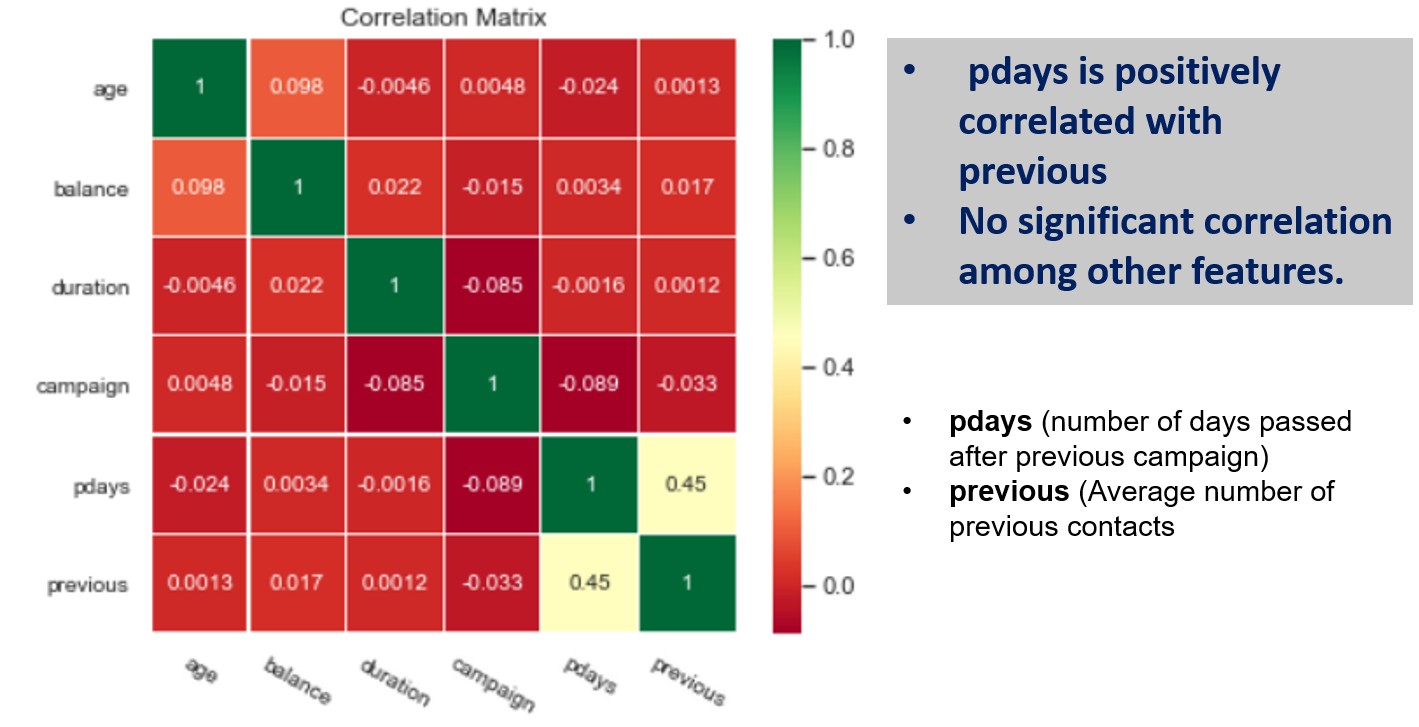
\includegraphics[width = 0.8\hsize]{./resources/img/fig_corr_matrix.png}
\caption{Heatmap plot of the correlation matrix of the numerical features.} 
\label{fig:corr_matrix}
\end{figure}








